%--------------------------------------------------------------------------------------
%	PACKAGES, THEMES and COMMANDS
%----------------------------------------------------------------------------------------
\documentclass[aspectratio=169,xcolor=dvipsnames]{beamer}

\usetheme{Boadilla}
\usecolortheme{dolphin}
\setbeamertemplate{caption}[numbered]

\usepackage{utilities/slashbox}
\usepackage{amsbsy}
\usepackage[dvipsnames]{xcolor}
\usepackage{tikz}
\usetikzlibrary{arrows}
\usepackage[skip=2pt]{caption}

\newcommand\mytextbullet{\leavevmode%
\usebeamertemplate{itemize item}\hspace{.5em}}
\DeclareMathOperator{\E}{\mathbb{E}}
\newcommand{\veca}{\boldsymbol{a}}
\newcommand{\vecalpha}{\boldsymbol{\alpha}}
\newcommand{\setn}{\mathcal{N}}
\newcommand{\seta}{\mathcal{A}}
\newcommand{\setc}{\mathcal{C}}
\newcommand{\vecx}{\textbf{x}}
\newcommand{\vecy}{\textbf{y}}
\newcommand{\matx}{\textbf{X}}
\newcommand{\maty}{\textbf{Y}}
\newcommand{\veceta}{\boldsymbol{\eta}}
\newcommand{\vectheta}{\boldsymbol{\theta}}



%----------------------------------------------------------------------------------------
%	TITLE PAGE
%----------------------------------------------------------------------------------------

\title[Nowicki and Snijders '01]{Estimation and Prediction for Stochastic Blockstructures} \subtitle{Krzysztof Nowicki and Tom A. B. Snijders, 2001.}
\author[andrea.teruzzi@proton.me] {Andrea Teruzzi}
%\author{andrea.teruzzi@studbocconi.it}
\date[VSI – BayesLab]{July 4, 2022} 

% BIDSA BAYES LAB


%----------------------------------------------------------------------------------------
%	INTRODUCTION SLIDES
%----------------------------------------------------------------------------------------

\begin{document}

\begin{frame}
    \titlepage
\end{frame}
%----------------------------------------------------

\AtBeginSection[]
{
  \begin{frame}
    \frametitle{Table of Contents}
    \tableofcontents[currentsection,hideothersubsections,currentsubsection]
  \end{frame}
}

%----------------------------------------------------------------------------------------
%	PRESENTATION SLIDES
%----------------------------------------------------------------------------------------

%------------------------------------------------
\section{Introduction and Preview}
%------------------------------------------------
\begin{frame}{Introduction and Preview}
\begin{itemize}
    \item The paper extends the approach of Nowicki and Snijders (1997) to a larger class of relational data.
    
    \item The goal of the paper is defining a general approach for partitioning a set of individuals into classes, given a set of pairwise relations.
    
    \item In order to do so we need:
        
        \addtolength{\itemindent}{12pt}
        
        \item[$\blacktriangleright$] Set
        
        \item[$\blacktriangleright$] Probability law
        
        \item[$\blacktriangleright$] Inference on the probability law (Bayesian)
\end{itemize}
\end{frame}

%------------------------------------------------
%------------------------------------------------
\section{Discrete Relational Data}
%------------------------------------------------
%\begin{frame}{Relational Data: graphs}
%
%\begin{block}<1->{Definition}
%A \textbf{graph} is a pair $g=(V, e)$, where \textit{V} is the set of vertices and \textit{e} is the set of edges. 
%\end{block}
%
%
%\begin{block}<2->{Definition}
%A \textbf{random graph} $G=(V, E)$ is a graph whose edges have a probability $p\geq 0$ to exist. We can see random graphs as \textbf{random variables} whose realization are graphs.
%\end{block}
%\uncover<3->{
%Generally, we can have particular subcategories of graphs:
%\begin{itemize}
%    \item \textbf{Graphs} (i.e. undirected graphs)
%    \item \textbf{Digraphs}
%    \item \textbf{Tournaments}
%    \item etc.
%\end{itemize}}
%\end{frame}

%------------------------------------------------
\begin{frame}{Example}

\begin{columns}
    % Column 1
    \begin{column}{.3\textwidth}
        \begin{center}
        \vspace{-29pt}
        Set of vertices V\\
        \vspace{5pt}
        \begin{tikzpicture}[scale = 1.7]
        \tikzset{vertex/.style = {shape=circle,draw,minimum size=1.5em}}
        % vertices
        \node[vertex] (1) at  (0,0) {$1$};
        \node[vertex] (2) at  (2,0) {$2$};
        \node[vertex] (3) at  (0,-2) {$3$};
        \node[vertex] (4) at  (2,-2) {$4$};
        \end{tikzpicture} 
        \end{center}
    \end{column}
    
    % Column 2
    \begin{column}{.3\textwidth}
        \begin{center}
        \vspace{-30pt}
        Graph $G$ (e.g. assistance)\\
        \begin{tikzpicture}[scale = 1.3]
        \tikzset{vertex/.style = {shape=circle,draw,minimum size=1.5em}}
        \tikzset{edge/.style = {very thick}}
        % vertices
        \node[vertex] (1) at  (0,0) {$1$};
        \node[vertex] (2) at  (2,0) {$2$};
        \node[vertex] (3) at  (0,-2) {$3$};
        \node[vertex] (4) at  (2,-2) {$4$};
        %edges
        \draw[edge] (1) to (2);
        \draw[edge] (2) to (3);
        \draw[edge] (4) to (3);
        \draw[edge] (4) to (1);
        \end{tikzpicture} 
        \vspace{5pt}
        %----------------------------------
        Digraph $D$ (e.g. friendship)\\
        \begin{tikzpicture}[scale = 1.3]
        \tikzset{vertex/.style = {shape=circle,draw,minimum size=1.5em}}
        \tikzset{edge/.style = {->,> = latex', very thick, draw = Violet}}
        % vertices
        \node[vertex] (1) at  (0,0) {$1$};
        \node[vertex] (2) at  (2,0) {$2$};
        \node[vertex] (3) at  (0,-2) {$3$};
        \node[vertex] (4) at  (2,-2) {$4$};
        %edges
        \draw[edge] (1) to (2);
        \draw[edge] (1.260) to (3.100);
        \draw[edge] (4.125) to (1.325);
        \draw[edge] (3.80) to (1.280);
        \draw[edge] (4) to (3);
        \draw[edge] (1.305) to (4.145);
        \end{tikzpicture}
        \end{center}
    \end{column}
    
    % Column 3    
    \begin{column}{.3\textwidth}
    \vspace{-10pt}
    \begin{center}
        $G$ and  $D$ combined 
        \vspace{10pt}
        \begin{tikzpicture}[scale = 1.8]
        \tikzset{vertex/.style = {shape=circle,draw,minimum size=1.5em}}
        \tikzset{vertexc/.style = {shape=circle,draw,minimum size=1.5em,fill = Periwinkle }}
        \tikzset{vertexcc/.style = {shape=circle,draw,minimum size=1.5em,fill = yellow }}
        \tikzset{edge/.style = {very thick}}
        \tikzset{edged/.style = {->,> = latex',  very thick, draw = Violet}}
        % vertices
        \node[vertex] (1) at  (0,0) {$1$};
        \node[vertex] (2) at  (2,0) {$2$};
        \node[vertex] (3) at  (0,-2) {$3$};
        \node[vertex] (4) at  (2,-2) {$4$};
        \node[vertexc] (5) at  (0,0) {$1$};
        \node[vertexcc] (6) at  (2,0) {$2$};
        \node[vertexc] (7) at  (0,-2) {$3$};
        \node[vertexc] (8) at  (2,-2) {$4$};
        
        %edges undirected
        \draw[edge] (1.348) to (2.192);
        \draw[edge] (1) to (4);
        \draw[edge] (2) to (3);
        \draw[edge] (4.192) to (3.348);
        \draw[edge] (4) to (1);
        %edges directed
        \draw[edged] (1.12) to (2.168);
        \draw[edged] (4.115) to(1.335);
        \draw[edged] (1.295) to (4.155);
        \draw[edged] (4.168) to (3.12);
        \draw[edged] (1.258) to (3.102);
        \draw[edged] (3.78) to (1.282);
        \end{tikzpicture} 

    \end{center}
    \end{column}
    
\end{columns}
\end{frame}
%------------------------------------------------
\begin{frame}{Relational Data: dyadic relations I}
\begin{itemize}
    \item Given a set of $n$ vertices labeled $1, \dots ,n$, we define the \textbf{set of pairs} for which the probability model applies:
    $$\setn \subset \setn_0 = \{ (i,j) \in \{1, \dots ,n\}^2| i\neq j\}$$ 
     \vspace{-15pt}
    $$ e.g. \quad \setn = \{(1,2), (1,3), (1,4), (2,3), (2,4), (3,4) \} $$
    
    We assume $\setn$ to be symmetric i.e. $(i, j) \in \setn \iff (j, i) \in \setn$.
    
    \vspace{5pt}
    \item The relation from vertex $i$ to vertex $j$ takes a value from the the finite set:
    $$ \vecalpha = \{ a_1, a_2, \dots, a_R \}$$
     \vspace{-15pt}
    $$ e.g. \quad \vecalpha = \{0, A, F, AF \} \quad R=4 $$
    
    The aims of our probability model is take into account the mutual dependence of relation from $i$ to $j$ and from $j$ to $i$. We define the \textbf{set of dyadic relations}:
    $$
    \vecalpha^2 = \{ \veca = (a_t, a_v) | a_t, a_v \in \vecalpha\}
    $$
\end{itemize}
\end{frame}
%------------------------------------------------
\begin{frame}{Relational Data: dyadic relations II}
\begin{itemize}
\item We call $\seta \subset \vecalpha^2$ the \textbf{alphabet} of pairwise relations. For every $(i,j) \in \setn$ exists $\veca = (a_t, a_v) \in \seta$ describing the dyadic relation of between $i$ and $j$.
\item An important operator on $\seta$ is the \textbf{reflection operator}:
$$ 
\pi(x, y) = (y, x)
$$
\vspace{-15pt}
\begin{itemize}%
    \setlength\itemsep{0.4em}
    \item $\seta$ is \textbf{closed under reflection}
    \item $\seta_0 = \{\veca\in\seta | \pi(\veca)=\veca\}$ is the set of symmetric relations
    \item $\seta_1 = \{\veca\in\seta | \pi(\veca)\neq\veca\}$ is the set of asymmetric relations
    \item $\seta = \seta_0\cup \seta_1$ and $\seta_0\cap \seta_1 = \varnothing$
    \item To avoid redundancy, $\seta_1$ can be partitioned into 2 disjoint half subsets such that $\seta_1 = \seta_{10}\cup\seta_{11},\, \seta_{10}\cap\seta_{11} = \varnothing$ and $\, \pi(\seta_{10}) = \seta_{11}$
    \item We define $\seta' = \seta_{0} \cup \seta_{10}$ 
    \item We denote $r = |\seta|,\, r_0 = |\seta_0|, \,r_1 = \frac{1}{2}|\seta_1| = |\seta_{10}| = |\seta_{11}|$
    
\end{itemize}
\end{itemize}
\end{frame}
%------------------------------------------------
\begin{frame}{Example}
    \begin{columns}
    % Column 1
    \begin{column}{.4\textwidth}
        \vspace{-10pt}
    \begin{center}
        $G$ and  $D$ combined 
        \vspace{10pt}
        \begin{tikzpicture}[scale = 1.8]
        \tikzset{vertex/.style = {shape=circle,draw,minimum size=1.5em}}
        \tikzset{vertexc/.style = {shape=circle,draw,minimum size=1.5em,fill = Periwinkle }}
        \tikzset{vertexcc/.style = {shape=circle,draw,minimum size=1.5em,fill = yellow }}
        \tikzset{edge/.style = {very thick}}
        \tikzset{edged/.style = {->,> = latex',  very thick, draw = Violet}}
        % vertices
        \node[vertex] (1) at  (0,0) {$1$};
        \node[vertex] (2) at  (2,0) {$2$};
        \node[vertex] (3) at  (0,-2) {$3$};
        \node[vertex] (4) at  (2,-2) {$4$};

        %edges undirected
        \draw[edge] (1.348) to (2.192);
        \draw[edge] (1) to (4);
        \draw[edge] (2) to (3);
        \draw[edge] (4.192) to (3.348);
        \draw[edge] (4) to (1);
        %edges directed
        \draw[edged] (1.12) to (2.168);
        \draw[edged] (4.115) to(1.335);
        \draw[edged] (1.295) to (4.155);
        \draw[edged] (4.168) to (3.12);
        \draw[edged] (1.258) to (3.102);
        \draw[edged] (3.78) to (1.282);
        \end{tikzpicture} 

    \end{center}
    \end{column}
    
    % Column 2
    \begin{column}{.5\textwidth}
        \begin{align*}
        & \setn = \{(1,2), (1,3), (1,4), (2,3), (2,4), (3,4) \}  \\ 
        & \vecalpha = \{0, A, F, AF \}\\ 
        & \\
        & \seta_0 =\{ (0,0), (A,A),  (F,F), (AF,AF)\}  \\  
        & \seta_1 =\{ (0,F), (F,0) (A,AF), (AF,A) \} \\ \
        & \seta_{10}=\{(0,F), (A,AF) \} \\ 
        & \seta_{11}=\{(F,0), (AF,A) \} \\ 
        & \\
        & r = |\seta|= 8 \\
        & r_0 = |\seta_0|= 4 \\
        & r_1 = 1/2|\seta_1| = |\seta_{10}|= |\seta_{11}|=2 \\
        \end{align*} 
        
    \end{column}

    
\end{columns}
\end{frame}

%------------------------------------------------
\begin{frame}{{Relational Data: Colored Relational Structure}}

The second aspect of the structure is a \textbf{discrete vertex characteristic}. The set of vertices $\{1, \dots ,n\}$ is partitioned into $c$ colors $1, \dots, c$ and we denote the set of colors $\setc = \{1, \dots ,c\}$.

\vspace{5pt}
\begin{block}{Definition}
It is called \textbf{colored relational structure} a set $\setn$ of ordered pairs of vertices between which relations are given, with the vertices belonging to $c$ categories stored in the vector $\vecx = (x_i)^n_{i=1}$ with $x_i \in \setc$ and with a relational structure where the dyadic relations $\vecy = (y_{ij})_{(i,j) \in \setn}$ take values in $\seta$.\\
 We consider a stochastic setting and we denote the random adjacency matrix and the random vector of colors by $(\maty, \matx)$.
\end{block}

\vspace{5pt}
In our particular framework,  we will consider $\maty = \vecy$ observed, but $\matx$ unknown (posteriori blockmodelling).

\end{frame}
%------------------------------------------------

%------------------------------------------------
%------------------------------------------------
\section{Stochastic Structures with Randomly Colored Vertices}
%------------------------------------------------
\begin{frame}{Stochastic blockmodel: $P(X)$ }

The ultimate goal of our analysis is specify a probability model for colored relational structures. In particular we are interested in:
\begin{itemize}
    \item The predictive density $P(\matx|\vecy)$
    \item Estimate the vector of parameters of the models.
\end{itemize}

Assume that the random colors $X_i$ are iid random variables with probability:
    $$ P(X_i=k)=\theta_k \quad k \in \setc $$

and the joint distribution of $\matx$ to be:
\begin{gather*}
    P(X=x) = \theta_1^{m_1} \dots \theta_c^{m_c}  \\
    m_k = \sum ^n _{i=1} I(x_i = k)
\end{gather*}
The vector $(m_k)_{k \in \setc}$ is \textbf{sufficient statistic} for the probability law of $X$.
    
\end{frame}
%------------------------------------------------
\begin{frame}{Stochastic blockmodel: $P(Y|x)$  I}

Given the vector of colors $\matx = \vecx$, the random vectors $\maty_{ij}$ for $(i,j) \in \setn$ with $i <j$ are \textbf{independent} with probabilities:
$$
P(\maty_{ij}=\veca| \matx = \vecx) = \eta_{\veca}(x_i, x_j) \quad \text{for } \ \veca \in \seta \text{ and } x_i, x_j \in \setc
$$  \vspace{-15pt}
$$
e.g. \quad \eta_{(AF,A)}(x_2=blue, x_3=red)
$$

and the array $\veceta$ of \textbf{color-dependent dyad probabilities} satisfies: 
$$
\sum_{\veca \in \seta} \eta_{\veca}(k,h) = 1 \quad \text{for all } k,h \in \setc
$$

Because $y_{ij}=\pi(y_{ji})$, the probabilities $\veceta$ must be \textbf{invariant} with respect to the reflection operator :
$$
\eta_{\veca}(k,h) = \eta_{\pi(\veca)}(h,k)
$$

\vspace{5pt}
which implies a \textbf{redundancy in parameters} $\eta_a(k,h)$.
\end{frame}
%------------------------------------------------
\begin{frame}{Stochastic blockmodel: $P(Y|x)$  II}

    A non-redundant parameterization is obtained as follows:
    $$
    \begin{cases}
      \eta_{\veca}(k,h) & \text{for }\veca\in\seta \text{ and } k<h \\
      \eta_{\veca}(k,k) & \text{for }\veca\in\seta'\text{ and } k \in \setc \\
   \end{cases}
    $$
    
    The \textbf{conditional joint distribution} $P(\vecy|\vecx)$ is given by:
    $$
    P(y|\vecx,\boldsymbol{\theta}, \veceta) =
    \Bigg( \prod_{\veca\in\seta}\prod_{1\leq k<h \leq c}(\eta_{\veca}(k,h))^{e_{\veca}(k, h)} \Bigg) \times
    \Bigg(\prod_{\veca\in\seta'}\prod_{k=1}^c(\eta_{\veca}(k,k))^{e_{\veca}(k, k)}\Bigg)
    $$
    where $e_{\veca}(k, h)$ counts the number of relations  of type $\veca$ from vertices of color $k$ to vertices of color $h$ and is a \textbf{sufficient statistic}.

\end{frame}
%------------------------------------------------
\begin{frame}{Stochastic blockmodel}

The stochastic blockmodel is then given by the joint distribution of $(\maty, \matx)$:
    \begin{align*}
        P(\vecy, \vecx|\,\boldsymbol{\theta}, \veceta) = &\hspace{3pt} P(\vecx)\times P(\vecy |\,\vecx, \boldsymbol{\theta}, \veceta) \\
        =& \hspace{3pt} \theta_1^{m_1}  \times \dots \times \theta_c^{m_c} \\
        &\times \Bigg(\prod_{\veca\in\seta}\prod_{1\leq k<h \leq c}(\eta_{\veca}(k,h)^{e_{\veca}(k, h))}\Bigg)\\
        &\times\Bigg(\prod_{\veca\in\seta'}\prod_{k=1}^c(\eta_{\veca}(k,k))^{e_{\veca}(k, k)}\Bigg)
    \end{align*}

    Because our model consider a stochastic structure $(\maty, \matx)$, with $\maty$ observed and $\matx$ latent variable, the probability of observing edge pattern $\vecy$ is:
    $$
    P(\vecy | \, \boldsymbol{\theta}, \veceta) = \sum_{\vecx \in \setc^n} P(\vecy, \vecx | \, \boldsymbol{\theta}, \veceta)
    $$


\end{frame}
%------------------------------------------------
\begin{frame}{Bayesian posteriori blockmodelling}
From the stochastic blockmodel:

\begin{itemize}
    \item We assume a prior density $f(\vectheta,\veceta)$ for the parameters $(\vectheta,\veceta)$, which we can update using $\vecy$ and \textbf{inference about the parameters}:
    $$
    f(\vectheta,\veceta| \, \vecy) = \sum_{x} f(\vectheta,\veceta, \vecx| \, \vecy)
    $$
    \item The \textbf{recovery of the block structure} is based on the posterior predictive distribution of of $\matx$:
    $$
    P(x| \, y) = \int  f(\vectheta,\veceta, \vecx| \, \vecy) d\vectheta d\veceta
    $$\\
    
    \item[$\Longrightarrow$] \textbf{Gibbs sampling} is used to obtain the conditional distribution $f(\vectheta,\veceta, \vecx| \, \vecy)$, which we need to solve both problems.
 \end{itemize}

\end{frame}
%------------------------------------------------
%------------------------------------------------
\section{Identifiability and Invariant Parameters}
%------------------------------------------------
\begin{frame}{Identifiability}

The parameters $(\vectheta, \veceta)$ in the joint distribution $f(\vectheta, \veceta, \vecx, \vecy$) \textbf{are not identifiable}. What matters is the partition defined by $\vecx$, not the colors labels $1, \dots, c$. \\

\vspace{10pt}
In particular, let $\mathcal{S}$ denote the group of permutation of $\{1, \dots ,c\}$ and define $h_s(\cdot)$ and $s(\cdot)$ such that:
    \begin{gather*}
       P(\maty =\vecy | \, \vectheta, \veceta ) = P(\maty =\vecy | \, h_s(\vectheta, \veceta) )\\
       s(\vecx) = ( s(x_1), \dots, s(x_n))
    \end{gather*}
    for every permutation $s \in \mathcal{S}$.  The transformation preserves the partition of the vertices and it implies:
    $$
    P(\vecx | \, \vecy, \vectheta, \veceta) = P(s(\vecx) | \, \vecy, h_s(\vectheta, \veceta))
    $$

\end{frame}
%------------------------------------------------

\begin{frame}{Invariance I}
Because the model is invariant under the relabelling of the colors, \textbf{when the prior distribution is invariant, then the posterior is invariant}:
    $$
    P(X_i=k| \, \vecy) = 1/c 
    $$
independently from $k$.  We can deal with the invariance problem in some ways: 

\begin{enumerate}
    \item  Put \textbf{restrictions} on the parameters
    $$
    e.g. \quad \theta_1 < \theta_2 \dots < \theta_c
    $$
    However this approach is not always applicable and it may require some prior information (informative prior).
\end{enumerate}
\end{frame}
%------------------------------------------------
\begin{frame}{Invariance II}
\begin{enumerate}
    \stepcounter{enumi}
    \item Consider the \textbf{posterior distribution of functions of} $(\vectheta, \veceta, \matx )$ \textbf{that are invariant} with respect to relabelling.  In particular we consider:
    \vspace{5pt}
    \addtolength{\itemindent}{24pt}
        \item[$\blacktriangleright$] $I\{X_i = X_j\}$
        
        \item[$\blacktriangleright$] $\eta_{\veca}(X_i,X_j) = \displaystyle\sum_{1\leq k, h\leq c}\eta_{\veca}(k,h) I\{X_i = k, X_j = h\}$
    \addtolength{\itemindent}{-24pt}
    \vspace{5pt}
    
    \item[] which are invariant w.r.t. the transformations $ h_s(\vectheta, \veceta)$ and $s(\matx)$.
    
    \item[] We can apply the expectation to these functions and find the following matrix and the three-way array :
    $$
    \bigg(P(X_i=X_j | \, \vecy)\bigg)_{1\leq i \neq j \leq n}
    $$
    $$
    \bigg( \E(\eta_{\veca}(X_i,X_j)|y\bigg)_{1\leq i \neq j \leq n, \, \veca \in \seta'}
    $$
\end{enumerate}

\end{frame}
%------------------------------------------------
\begin{frame}{Example}
    \begin{columns}
    % Column 1
    \begin{column}{.4\textwidth}
        \vspace{-10pt}
    \begin{center}
        $G$ and  $D$ combined 
        \vspace{10pt}
        \begin{tikzpicture}[scale = 1.8]
        \tikzset{vertex/.style = {shape=circle,draw,minimum size=1.5em}}
        \tikzset{vertexc/.style = {shape=circle,draw,minimum size=1.5em,fill = Periwinkle }}
        \tikzset{vertexcc/.style = {shape=circle,draw,minimum size=1.5em,fill = yellow }}
        \tikzset{edge/.style = {very thick}}
        \tikzset{edged/.style = {->,> = latex',  very thick, draw = Violet}}
        % vertices
        \node[vertexc] (1) at  (0,0) {$1$};
        \node[vertexcc] (2) at  (2,0) {$2$};
        \node[vertexc] (3) at  (0,-2) {$3$};
        \node[vertexc] (4) at  (2,-2) {$4$};
        
         % vertices 2
        \node[vertexcc] (1) at  (0,0) {$1$};
        \node[vertexc] (2) at  (2,0) {$2$};
        \node[vertexcc] (3) at  (0,-2) {$3$};
        \node[vertexcc] (4) at  (2,-2) {$4$};

        %edges undirected
        \draw[edge] (1.348) to (2.192);
        \draw[edge] (1) to (4);
        \draw[edge] (2) to (3);
        \draw[edge] (4.192) to (3.348);
        \draw[edge] (4) to (1);
        %edges directed
        \draw[edged] (1.12) to (2.168);
        \draw[edged] (4.115) to(1.335);
        \draw[edged] (1.295) to (4.155);
        \draw[edged] (4.168) to (3.12);
        \draw[edged] (1.258) to (3.102);
        \draw[edged] (3.78) to (1.282);
        \end{tikzpicture} 

    \end{center}
    \end{column}
    
    % Column 2
    \begin{column}{.5\textwidth}
    \begin{center}
    \vspace{-10pt}
    
    $I\{X_i = X_j\}$ \\ \vspace{10pt}
     \linethickness{1pt}
    \setlength{\arrayrulewidth}{1pt}
    \begin{tabular}{|c|c|c|c|c|}
    \hline
    \backslashbox{$X_i$}{$X_j$}  &   \textit{1}   &  \textit{2}  & \textit{3} & \textit{4} \\ \hline
                \textit{1}            &   -   &  0  & 1 & 1 \\ \hline
                \textit{2}            &   0   &  -  & 0 & 0 \\ \hline
                \textit{3}            &   1   &  0  & - & 1 \\ \hline
                \textit{4}            &   1   &  0  &  1 & - \\ \hline
    \end{tabular}

 
    \end{center}
    
    
  
   
    \end{column}

    
\end{columns}
\end{frame}

%-------------------------


%------------------------------------------------
%------------------------------------------------
\section{Gibbs Sampling for the Posterior Distribution}
%------------------------------------------------
\begin{frame}{Gibbs Sampler}
\begin{block}{Definition}
    \textbf{Gibbs Sampling} is a simulation method used to approximate a target posterior distribution. It is an iterative simulation scheme that, given a set of unknown random vectors, consists in drawing each random vector from its probability law conditioned on the values of all of the other random vectors.
\end{block}

\vspace{10pt}
We apply this scheme to $((\vectheta, \veceta), X_1, X_2, \dots, X_n)) $.  At each iteration, given the current values $(\vectheta^{(p)}, \veceta^{(p)}, \matx^{(p)})$:
\begin{enumerate}
    \item Draw $(\vectheta^{(p+1)}, \veceta^{(p+1)})$ from $f(\vectheta, \veceta | \, \matx^{(p)}, \vecy) $ 
    \item For each $i=1, \dots, n$: draw $X^{(p+1)}_i$ from $f(X_i| \vectheta^{(p+1)}, \veceta^{(p+1)}, (X_j^{(p+1)})_{j<i}, (X_k^{(p)})_{k>j} )$
\end{enumerate}

We are left to specify the full conditional distribution for these two steps.
\end{frame}
%------------------------------------------------
\begin{frame}{Step 1: Prior choice I}
For step 1, we need to specify the \textbf{prior distribution} $f(\vectheta, \veceta)$. If we do not have any particular prior information, it is also reasonable to assume \textbf{independence} between $\vectheta$ and $\veceta$.
 
\vspace{5pt}
\begin{itemize}
    \item For $\vectheta$ we use a \textbf{Dirichlet} $D(T_1,\dots, T_c)$.
        \addtolength{\itemindent}{12pt}
        
        \item[$\blacktriangleright$] $T_k = 1$ corresponds to uniform distribution
        
        \item[$\blacktriangleright$]  $T_k =T$ small when we think the true model has less classes than $c$
        
        \item[$\blacktriangleright$]  $T_k=T$ large when we think the true model has $c$ classes (e.g. $T=100c$)
        \addtolength{\itemindent}{-12pt}
\vspace{10pt}
    
    \item For $\veceta$ use a \textbf{Dirichlet} of parameters $E_{\veca}(k,h)$.
        \addtolength{\itemindent}{12pt}
        
        \item[$\blacktriangleright$] For $k<h$, $\veceta(k,h)=(\veceta_{\veca}(k,h))_{\veca \in \seta}$ is an unconstrained probability vector of dimension $r=|\seta|$.
\end{itemize}
\end{frame}
%------------------------------------------------
\begin{frame}{Step 1: Prior choice II}
\begin{itemize}
        \addtolength{\itemindent}{12pt}
        \item[$\blacktriangleright$] For $k=k$, $\veceta(k,k)$ is constrained to $\veceta_{\veca}(k,k) = \veceta_{\pi(\veca)}(k,k)$. We  define:
        $$
        \veceta^{(0)}_{\veca}(k,k) =
        \begin{cases} 
        \veceta_{\veca}(k,k) \quad \veca \in \seta_0 \\
        2\veceta_{\veca}(k,k) \quad \veca \in \seta_{10}
        \end{cases}
        $$
        transforming $\veceta(k,k)$ in a ($r_0+r_1$)-dimensional (note $r_0+r_1<r$) vectors without redundant elements for every $k \in \setc$.

         
        \item[$\blacktriangleright$] Set $E_{\veca}(k,h)=1$ for an invariant prior. 
\end{itemize}
The posterior distribution of $(\vectheta, \veceta)$ given $(\vecy, \vecx)$ is  is largely tractable:
\begin{gather*}
    (m_k + T_k)_{k \in \setc} \quad \text{ for } \vectheta \\
    (e_{\veca}(k,h) + E_{\veca}(k,h))_{\veca \in \seta } \quad \text{ for } \veceta(k,h), \, 1\leq k < h \leq c \\
    (e_{\veca}(k,k) + E_{\veca}(k,k))_{\veca \in \seta'} \quad \text{ for } \veceta^{(0)}(k,k), \, 1\leq k\leq c
\end{gather*}

We can approximate $\veceta_{\veca}(X_i,X_j)$ using the average of $\veceta^{(p)}_{\veca}(X_i,X_j)$ drawn from the Gibbs sampler.
    
\end{frame}
%------------------------------------------------
\begin{frame}{Step 2: $f(X_i| \vectheta, \veceta, \vecx_{-i})$}
From the probability law of the stochastic block-model $P(\vecy, \vecx | \vectheta, \veceta) $ we can derive:
$$
P(X_i = k|\, \vecy, \vectheta, \veceta, \{X_j\}_{j\neq i})= Q\theta_k\prod_{\veca\in\seta}\prod_{h=1}^c (\veceta_{\veca}(k, h))^{d_{\veca}(i, h)}
$$
with $d_{\veca}(i, k) = \sum_{j:(i,j)\in\setn} I\{y_{ij} = \veca\}I\{x_j=k\}$  counting number of dyadic relations of type $\veca$ from vertex $i$ to vertices of color $k$ and with $Q$ a constant not depending on $k$.\\ 
\vspace{15pt}
The \textbf{relative frequency} of $X^{(p)}_i=X^{(p)}_j$ over the Gibbs sampler can be used to \textbf{approximate the matrix of posterior predictive probabilities} $ (P(X_i=X_j | \, \vecy))_{1\leq i \neq j \leq n}$
\vspace{30pt}
\end{frame}
%------------------------------------------------
\begin{frame}{Adequacy of class structure}
We can build some parameters for evaluating the adequacy of the obtained class structure:
 
\begin{itemize}
    \item $I_y$ is the information of the observed relations with $c \geq 2$:
    $$
    I_y = -\frac{2}{|\setn|}\sum_{(i,j)\in\setn, i<j} log(\eta_{y_{ij}}(X_i, X_j))
    $$
    This value is small when $\veceta$ and $\matx$ determine to a large extent of the observed relations.
    \vspace{5pt}
    \item $H_x$ measures the extent to which the distribution of $\matx$ defines one clear-cut partition of vertices into classes.
    $$
    H_x = \frac{4}{n(n-1)}\sum_{i,j = 1}^n \pi_{ij}(1-\pi_{ij})
    $$
    with $\pi_{ij} = P(X_i=X_j|\,\vecy)$. If $H_x$ is small it relatively clear if pair of vertices are in the same class or not.
\end{itemize}
\end{frame}
%------------------------------------------------
\begin{frame}{Example – Adequacy parameters}

\begin{figure}
    \centering
    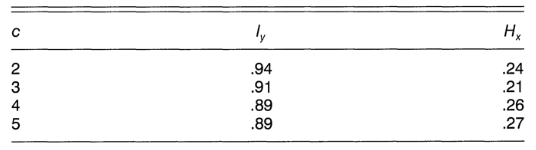
\includegraphics[keepaspectratio, height = 2.5cm]{utilities/adequacy_parameter.png}
    \caption{Parameter for the class structure for Kapferer's dataset}
    \label{fig:11}
\end{figure}
    
\end{frame}
%------------------------------------------------

\begin{frame}{Convergence and class assignment}
\vspace{-15pt}
To check to convergence of the Gibbs sampler:

\begin{itemize}
    \item Run multiple Gibbs sampler with different independent starting points and check that parameters $H_x $ and $I_y $ have similar values.
    
    \item For invariant prior, check that the the posterior predictive distribution of the sequence $\matx^{(p)}$ is uniform.
\end{itemize}
\vspace{10pt}

Assign vertices to classes:

\begin{itemize}
    \item For uniform prior, arbitrarily assign labels.
    
    \item For nonuniform prior, labels are identified by the prior.
\end{itemize}

\end{frame}
%------------------------------------------------
\begin{frame}{Example – Estimated posterior probabilities I}
\begin{figure}
    \begin{overprint}
    \centering
    \onslide<1> \centering 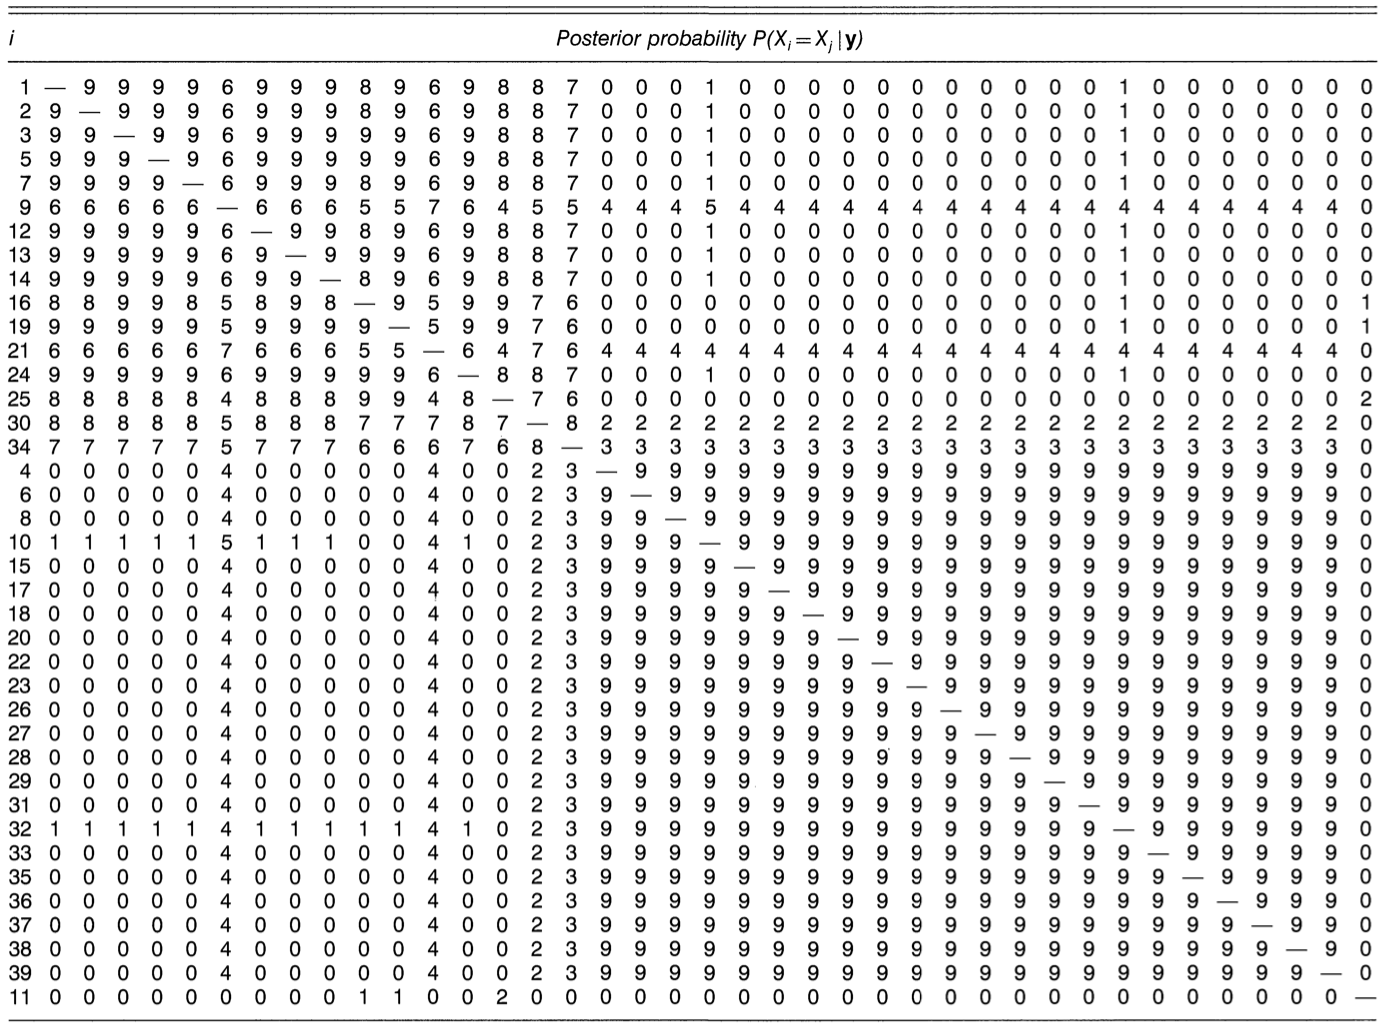
\includegraphics[keepaspectratio, height = 6.5cm]{utilities/exp_x.png}
    \caption{Estimated posterior probabilities $P(X_i=X_j| \, \vecy)$ for Kapferer's dataset}
    \label{fig:2}
    \setcounter{figure}{1}
    \onslide<2> \centering 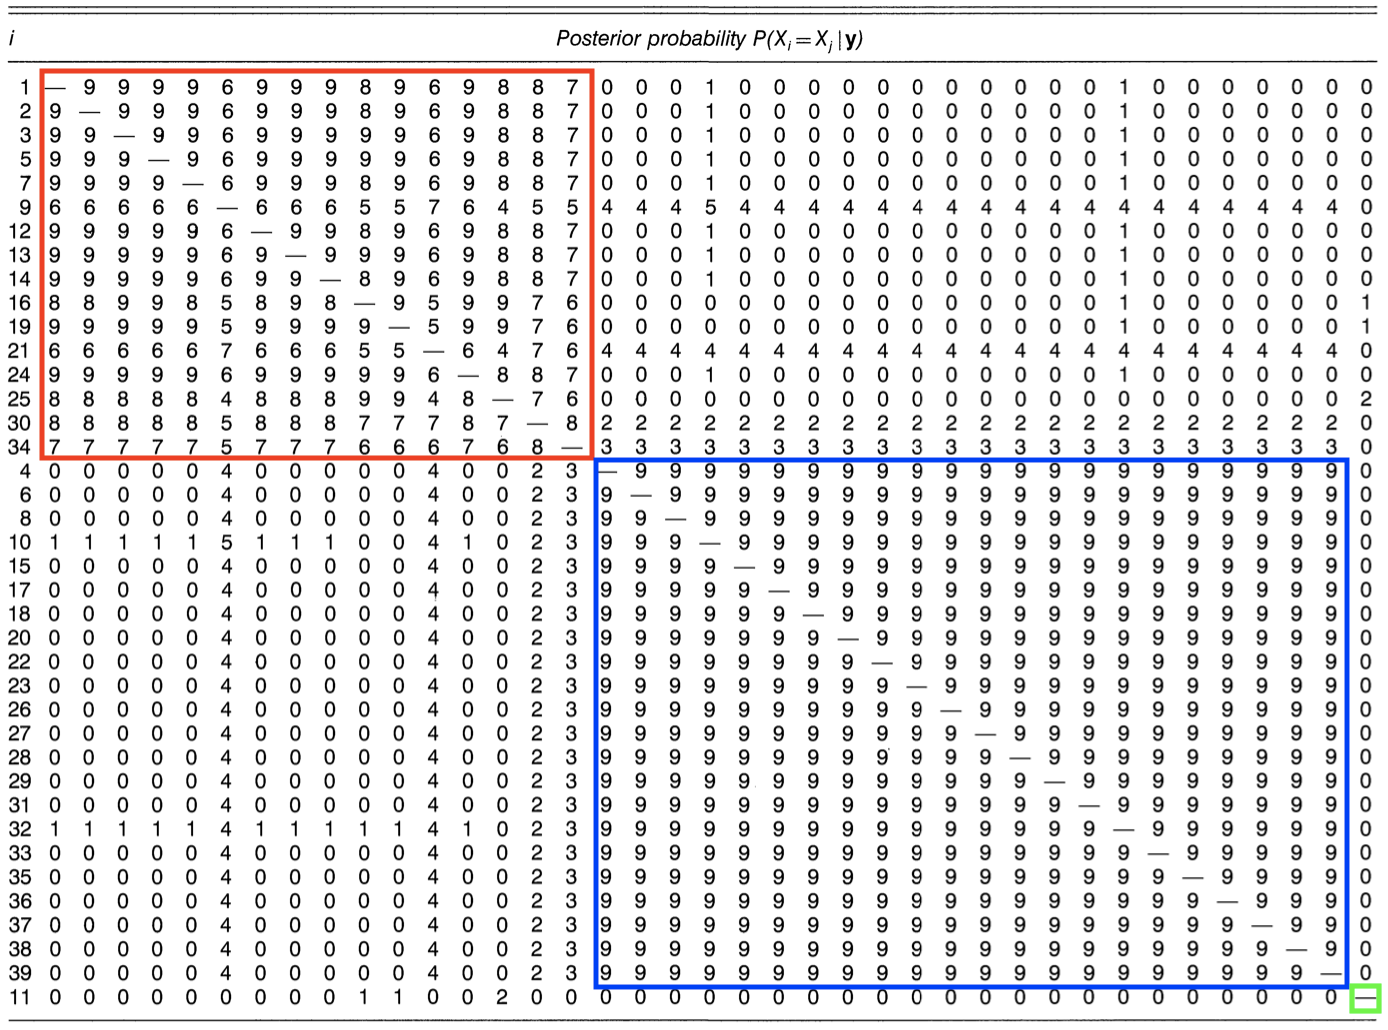
\includegraphics[keepaspectratio, height = 6.5cm]{utilities/exp_x_labels.png}  \caption{Estimated posterior probabilities $P(X_i=X_j| \, \vecy)$ for Kapferer's dataset}
    \label{fig:2}
    \end{overprint}
\end{figure}
    
\end{frame}
%------------------------------------------------
\begin{frame}{Example – Estimated posterior probabilities II}
\begin{figure}
    \centering
    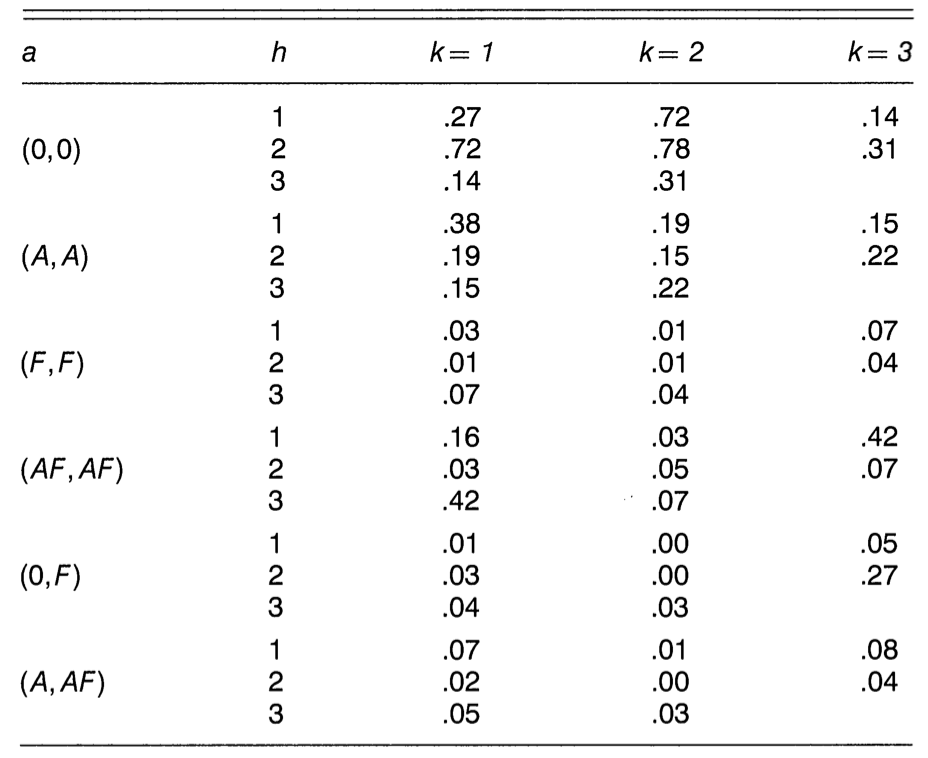
\includegraphics[keepaspectratio, height = 6.5cm]{utilities/exp_eta.png}
    \caption{Estimated posterior probabilities $\veceta_{\veca}(X_i,X_j)$ for Kapferer's dataset}
    \label{fig:3}
\end{figure}
    
\end{frame}
%------------------------------------------------

%------------------------------------------------
%------------------------------------------------
\begin{frame}[allowframebreaks]{Bibliography}
\bibliographystyle{alpha}
\nocite{nowicki_snijders_2001, nowicki_snijders_1997}
\bibliography{bibl.bib}
\end{frame}


%----------------------------------------------------------------------------------------

\end{document}